\documentclass[11pt,a4paper]{article}

\usepackage[utf8]{inputenc}
\usepackage[T1]{fontenc}
\usepackage{lmodern}
\usepackage[english]{babel}
\usepackage{microtype}
\usepackage[margin=2.25cm,headheight=15pt]{geometry}
\usepackage{graphicx}
\usepackage{booktabs}
\usepackage{tabularx}
\usepackage{longtable}
\usepackage{array}
\usepackage{enumitem}
\usepackage{xcolor}
\usepackage{amsmath}
\usepackage{float}
\usepackage[section]{placeins}
\usepackage{caption}
\usepackage{fancyhdr}
\usepackage{xurl}
\usepackage[colorlinks=true,linkcolor=black,urlcolor=blue!60!black,citecolor=black]{hyperref}

% Generated by generate_analysis.mjs. Do not edit by hand.
\newcommand{\PublicRows}{103,510}
\newcommand{\FullArchiveRows}{186,918}
\newcommand{\FlightDurationHours}{3.05}
\newcommand{\FlightEndMinute}{183.00747}
\newcommand{\FirstFixTime}{14:37:35}
\newcommand{\FirstFixMinutes}{8.59}
\newcommand{\LaunchTime}{14:38:56}
\newcommand{\AscentTime}{14:39:08}
\newcommand{\DescentTime}{16:15:22}
\newcommand{\LandingTime}{16:51:18}
\newcommand{\LaunchMinute}{9.9483}
\newcommand{\AscentMinute}{10.135}
\newcommand{\DescentMinute}{106.3683}
\newcommand{\LandingMinute}{142.3133}
\newcommand{\ApexMinute}{106.1833}
\newcommand{\ResetMinute}{142.65}
\newcommand{\StandbyDurationMin}{9.95}
\newcommand{\LaunchDurationS}{11.2}
\newcommand{\AscentDurationMin}{96.23}
\newcommand{\DescentDurationMin}{35.95}
\newcommand{\LandingDurationMin}{40.69}
\newcommand{\ApexGpsKm}{38.48}
\newcommand{\ApexGpsM}{38,480}
\newcommand{\ApexBaroKm}{28.873}
\newcommand{\MaxBaroKm}{28.881}
\newcommand{\ApexTime}{16:15:11}
\newcommand{\AltitudeDifferenceKm}{9.607}
\newcommand{\MaxClimb}{16.14}
\newcommand{\MaxDescent}{95.23}
\newcommand{\MeanAscent}{6.564}
\newcommand{\MeanDescent}{17.403}
\newcommand{\MaxGroundSpeed}{38.89}
\newcommand{\LaunchLatitude}{48.0879328}
\newcommand{\LaunchLongitude}{11.2960224}
\newcommand{\ApexLatitude}{47.9566112}
\newcommand{\ApexLongitude}{11.4497968}
\newcommand{\LandingLatitude}{47.879632}
\newcommand{\LandingLongitude}{11.692252}
\newcommand{\LaunchMapX}{1088.2618163}
\newcommand{\LaunchMapY}{-711.1660883}
\newcommand{\ApexMapX}{1089.1366218}
\newcommand{\ApexMapY}{-712.283056}
\newcommand{\LandingMapX}{1090.5159225}
\newcommand{\LandingMapY}{-712.9364901}
\newcommand{\LandingDistanceKm}{37.499}
\newcommand{\MaxRangeKm}{43.389}
\newcommand{\MinPressureHpa}{3.37}
\newcommand{\MinTemperatureC}{14.74}
\newcommand{\MaxTemperatureC}{35.72}
\newcommand{\BatteryMedianV}{3.856}
\newcommand{\BatteryPZeroFiveV}{3.718}
\newcommand{\BatteryPNinetyFiveV}{3.945}
\newcommand{\BatteryMinV}{3.088}
\newcommand{\BatteryMaxV}{4.668}
\newcommand{\BatteryOutlierRows}{8}
\newcommand{\MaxAccelerationG}{4.675}
\newcommand{\MaxAccelerationTime}{14:35:24}
\newcommand{\GoodCoralFrames}{630}
\newcommand{\CoralInvalidRows}{1,620}
\newcommand{\CoralInvalidPercent}{1.565}
\newcommand{\CoralTimeoutRows}{1,552}
\newcommand{\CoralFaultIntervals}{15}
\newcommand{\CoralLongestFaultS}{21.636}
\newcommand{\CoralTotalFaultS}{97.054}
\newcommand{\CloudMeanPercent}{12.704}
\newcommand{\CloudMedianPercent}{8.006}
\newcommand{\CloudPNinetyPercent}{33.202}
\newcommand{\CloudZeroPercent}{1.905}
\newcommand{\MedianSampleMs}{100}
\newcommand{\SamplePNinetyFiveMs}{109}
\newcommand{\LargestGapS}{8.673}
\newcommand{\SamplingStalls}{6}
\newcommand{\GenuineSamplingStalls}{5}
\newcommand{\LongestGenuineStallS}{1.299}
\newcommand{\FixThreePercent}{95.298}
\newcommand{\FixThreeRows}{98,643}
\newcommand{\ValidDownlinks}{200}
\newcommand{\InvalidDownlinks}{62}
\newcommand{\ReportedLostPackets}{180}
\newcommand{\DuplicateDownlinks}{0}
\newcommand{\RssiMedian}{-101.5}
\newcommand{\RssiMin}{-121}
\newcommand{\RssiMax}{-52}
\newcommand{\SnrMedian}{8.63}
\newcommand{\SnrMin}{-12}
\newcommand{\SnrMax}{13}
\newcommand{\InvalidDownlinkPercent}{23.66}
\newcommand{\SessionOneLastRangeKm}{45.06}
\newcommand{\SessionOneStopRangeKm}{24.78}
\newcommand{\SessionTwoStartRangeKm}{1}
\newcommand{\SessionTwoStartTime}{16:56:44}
\newcommand{\SessionTwoEndTime}{17:20:31}
\newcommand{\TtcCrcErrors}{64}
\newcommand{\TtcUnexpectedLengthPackets}{12}
\newcommand{\TtcCrcErrorsInWindow}{62}
\newcommand{\TtcUnexpectedLengthPacketsInWindow}{12}
\newcommand{\TtcFirstTime}{14:29:08}
\newcommand{\TtcLastTime}{17:20:31}
\newcommand{\BootGapS}{12.587}

\graphicspath{{figures/}{../../}}

\definecolor{lakitublue}{HTML}{165D8D}
\definecolor{lakituorange}{HTML}{E8871E}
\definecolor{lakitugreen}{HTML}{2A9D6F}
\definecolor{lakitured}{HTML}{C43D3D}
\definecolor{lakitugray}{HTML}{5B6573}
\definecolor{lightblue}{HTML}{EEF5FA}
\definecolor{lightorange}{HTML}{FFF5E8}
\definecolor{lightred}{HTML}{FCEEEE}

\hypersetup{
  pdftitle={Lakitu Flight Data Analysis - 28 July 2026},
  pdfauthor={Lakitu project team},
  pdfsubject={Post-flight telemetry analysis},
}
\captionsetup{font=small,labelfont=bf}
\setlist{nosep,leftmargin=1.6em}
\setlength{\parindent}{0pt}
\setlength{\parskip}{0.55em}
\renewcommand{\arraystretch}{1.16}
\emergencystretch=2em

\pagestyle{fancy}
\fancyhf{}
\fancyhead[L]{\small Lakitu post-flight analysis}
\fancyhead[R]{\small 28 July 2026}
\fancyfoot[C]{\thepage}
\renewcommand{\headrulewidth}{0.35pt}

\newcommand{\statusbox}[3]{%
  \begin{center}
  \fcolorbox{#1}{#2}{\begin{minipage}{0.92\linewidth}\textbf{#3}\end{minipage}}
  \end{center}
}
\newcommand{\sourcefile}[1]{\path{#1}}

\begin{document}

\begin{titlepage}
  \centering
  \vspace*{1.2cm}
  \includegraphics[width=0.24\textwidth]{scsd_lakitu_logo.png}\par
  \vspace{1.2cm}
  {\Huge\bfseries Lakitu Flight Data Analysis\par}
  \vspace{0.35cm}
  {\Large Stratospheric Balloon Flight - 28 July 2026\par}
  \vspace{1.1cm}
  \rule{0.78\textwidth}{0.6pt}\par
  \vspace{0.55cm}
  {\large Detailed post-flight telemetry, payload, health, and TT\&C report\par}
  \vspace{0.55cm}
  \rule{0.78\textwidth}{0.6pt}\par
  \vfill
  \begin{tabular}{rl}
    Primary window: & 14:29:00--17:32:00 CEST \\
    Primary records: & \PublicRows \\
    Window duration: & \FlightDurationHours\ h \\
    Report build: & 30 July 2026 \\
  \end{tabular}
  \vfill
  {\small Lakitu project team\par}
\end{titlepage}

\pagenumbering{roman}
\tableofcontents
\clearpage
\listoffigures
\listoftables
\clearpage
\pagenumbering{arabic}

\section{Executive summary}

This report analyses the coherent public on-board flight window from 14:29 to
17:32 CEST, containing \PublicRows\ rows sampled at a nominal 10~Hz. It also
uses the \FullArchiveRows-row merged archive for provenance and continuity
context and the two ground-station CSV sessions for received-link statistics.
The numerical summary, compact plotting tables, graph PDFs, and this report are
all generated from the same reproducible analysis script.

\statusbox{lakitublue}{lightblue}{Mission outcome. The platform reached a maximum GNSS altitude of \ApexGpsKm\ km at \ApexTime\ CEST. The mean measured ascent rate from the Ascent transition to apex was \MeanAscent\ m/s; the maximum measured downward speed was \MaxDescent\ m/s. The GNSS launch-to-landing displacement was \LandingDistanceKm\ km.}

\statusbox{lakituorange}{lightorange}{Primary performance discrepancy. At GNSS apex, the relative barometric altitude was \ApexBaroKm\ km, leaving a \AltitudeDifferenceKm\ km disagreement. This is too large to treat as ordinary sensor noise and requires calibration and atmospheric-model review.}

\statusbox{lakitured}{lightred}{Primary anomalies. The Coral link produced \CoralFaultIntervals\ timeout intervals and \CoralInvalidRows\ invalid telemetry rows (\CoralInvalidPercent\%). A power-on reset occurred at 16:51:39 CEST during Landing. No watchdog reset or non-Coral equipment fault was recorded.}

The flight-state machine transitioned Standby $\rightarrow$ Launch
$\rightarrow$ Ascent $\rightarrow$ Descent $\rightarrow$ Landing. It did not
enter Cruise. This is consistent with the recorded post-apex descent condition
being accepted before a 30-second cruise condition could be established, but it
should be checked against the intended mission-state requirements.

\section{Pre-flight preparation}

The released dataset does not include a signed field checklist, photographs of
the final integration state, or ground-station configuration records. The
pre-flight assessment below therefore distinguishes readiness demonstrated by
telemetry from preparation items that cannot be independently verified.

\begin{itemize}
  \item \textbf{On-board readiness.} During the public Standby interval, GPS,
  IMU, barometer, battery, SD, and LoRa remained enabled and no corresponding
  equipment fault was recorded. The battery rail was centred on
  \BatteryMedianV~V, and logging continued into Launch without a boot change.
  \item \textbf{Navigation readiness.} The first 3D GNSS fix was acquired at
  \FirstFixTime\ CEST, approximately 81 seconds before the
  Standby-to-Launch transition at \LaunchTime\ CEST. This provided a valid
  position and altitude reference before release.
  \item \textbf{Ground-station reference.} For session 1, the station position
  is taken as the CubeSat's initial valid GNSS position, consistent with the
  co-located field setup. This assumption is sufficient for the range
  reconstruction but is not a substitute for a logged station GNSS track.
  \item \textbf{Configuration records.} The archive does not prove that antenna
  attachment, connector retention, payload communications, reset-cause capture,
  or end-to-end packet decoding were checked immediately before flight. These
  items should be explicit, signed checklist gates for the next campaign.
\end{itemize}

\statusbox{lakitugreen}{lightblue}{Readiness assessment. The telemetry shows a stable on-board Standby period and a valid GNSS solution before release. The main evidential gap is operational configuration traceability rather than an observed pre-launch subsystem fault.}

\section{Data scope and provenance}

\subsection{Analysed sources}

\begin{table}[H]
\centering
\caption{Source files used in this report.}
\label{tab:sources}
\begin{tabularx}{\textwidth}{@{}p{0.25\textwidth}Xr@{}}
\toprule
Source & Role & Records \\
\midrule
\sourcefile{flight_data_2026-07-28_1429-1732_CEST.csv} & Primary, coherent public flight-analysis window & \PublicRows \\
\sourcefile{flight_data.csv} & Complete merged internal-memory archive; used for continuity and provenance checks & \FullArchiveRows \\
\sourcefile{telemetry_20260728_132651.csv} and \sourcefile{telemetry_20260728_165643.csv} & Ground-station decoded LoRa receptions and link measurements & 622 \\
\sourcefile{flight_data_audit.json} & Archive inventory, frame correlation, and source-file ledger & -- \\
\sourcefile{flight_anomaly_report.md} and \sourcefile{data_gaps.md} & Independent anomaly and gap reviews used for reconciliation & -- \\
\bottomrule
\end{tabularx}
\end{table}

The primary CSV is intentionally a time-window cut, not the whole internal
memory image. The full audit reports 340 CSV files, 1,104 RAW Coral frames,
1,104 converted PNGs, and 1,101 RAW frames with a successful matching CSV Coral
record. Photographs and RAW image content are outside this report's scope.

\subsection{Time basis}

The firmware stores GNSS time as \texttt{HHMMSS} without a calendar date. The
date 2026-07-28 therefore comes from archive provenance, not from a GNSS date
field. CEST is UTC+2 for this flight, so the public window corresponds to
12:29:00--15:32:00 UTC.

Within each run of identical one-second GNSS timestamps, this analysis uses the
STM32 HAL tick to interpolate a sub-second plotting coordinate. Interpolation
is restarted after an OBC boot because \texttt{record\_timestamp\_ms} resets.
Displayed event times retain the authoritative GNSS second. This method avoids
treating the HAL tick as continuous across the boot-5 to boot-6 reset.

\subsection{Units and interpretation}

\begin{table}[H]
\centering
\caption{Principal field transformations.}
\label{tab:scales}
\begin{tabularx}{\textwidth}{@{}lXl@{}}
\toprule
CSV field & Transformation & Report unit \\
\midrule
\texttt{gps\_lat\_e7}, \texttt{gps\_lon\_e7} & divide by $10^7$ & degrees \\
\texttt{gps\_alt\_cm}, \texttt{baro\_alt\_cm} & divide by 100 & m \\
\texttt{gps\_speed\_cms}, \texttt{gps\_vel\_down\_cms} & divide by 100; vertical plots negate down velocity & m/s \\
\texttt{imu\_accel\_*\_mg} & divide by 1,000 & g \\
\texttt{imu\_gyro\_*\_mdps} & divide by 1,000 & deg/s \\
\texttt{baro\_pressure\_pa} & divide by 100 & hPa \\
\texttt{baro\_temp\_centi\_c} & divide by 100 & $^\circ$C \\
\texttt{batt\_voltage\_mv} & divide by 1,000 & V \\
\texttt{coral\_block\_hex[4..5]} & little-endian Q16 divided by 65,535 & cloud fraction \\
\bottomrule
\end{tabularx}
\end{table}

The barometric altitude is relative to the Standby ground baseline; it is not
an independent geodetic altitude. The MS5607 temperature channel is a sensor
temperature used in pressure compensation and must not be presented as a
calibrated ambient-air temperature.

\section{Flight timeline and state-machine behaviour}

\begin{table}[H]
\centering
\caption{Recorded flight-state transitions. Positive vertical-down velocity denotes descent.}
\label{tab:timeline}
\begin{tabular}{@{}llllrrr@{}}
\toprule
CEST & From & To & Elapsed & GNSS alt. (m) & Baro alt. (m) & $v_D$ (m/s) \\
\midrule
\LaunchTime & Standby & Launch & 9:56 & 580 & 10.50 & $-3.82$ \\
\AscentTime & Launch & Ascent & 10:08 & 652 & 65.82 & $-7.55$ \\
\DescentTime & Ascent & Descent & 1:46:22 & 37,935 & 28,668.28 & 80.50 \\
\LandingTime & Descent & Landing & 2:22:18 & 753 & 170.28 & 5.18 \\
\bottomrule
\end{tabular}
\end{table}

The state durations in the public window were \StandbyDurationMin\ min in
Standby, \LaunchDurationS\ s in Launch, \AscentDurationMin\ min in Ascent,
\DescentDurationMin\ min in Descent, and \LandingDurationMin\ min in Landing.
Cruise duration was zero. State persistence was effective: after the power-on
reset, the first boot-6 record remained in Landing instead of reverting to
Standby.

\begin{figure}[H]
\centering
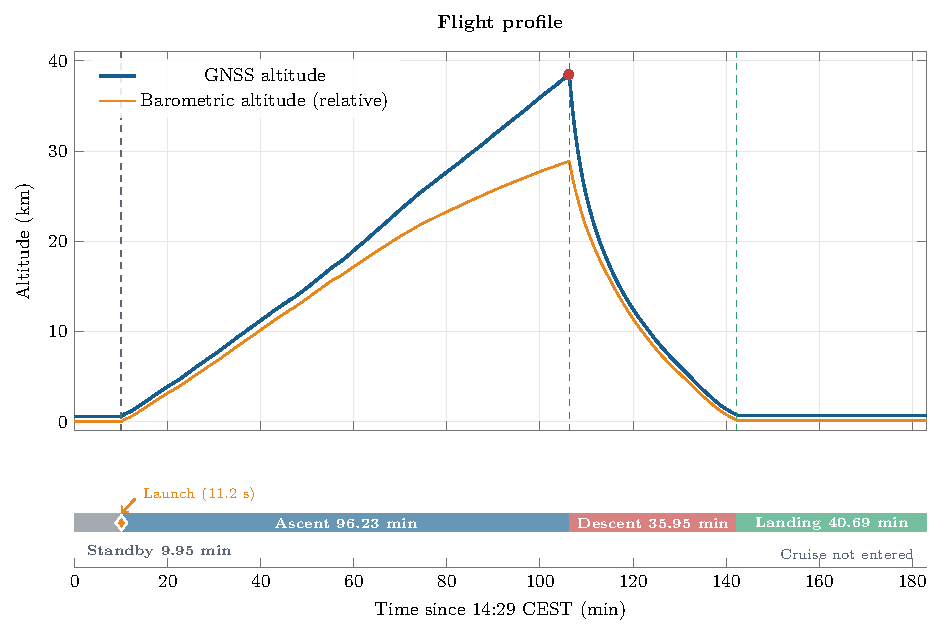
\includegraphics[width=\textwidth]{flight_profile.pdf}
\caption{Flight profile.}
\label{fig:profile}
\end{figure}

Figure~\ref{fig:profile} plots five-second medians of GNSS and relative
barometric altitude. Vertical lines mark the recorded phase transitions, and
each lower-band rectangle begins and ends at the corresponding transition time.
The duration is printed on or beside each band. The 11.2-second Launch state is
identified by a diamond because its true interval is too narrow for a legible
label at the full-flight scale; Cruise was not entered. Extrema and event values
reported in the text and tables are calculated from the full-rate rows.

The GNSS profile is consistent with a sustained balloon ascent followed by a
sharp burst/descent transition. The Ascent-to-Descent change occurs roughly
11 seconds after the maximum GNSS altitude record because the descent rule is
debounced. A distinct float interval is not visible in the state record.

\section{Altitude, velocity, and inertial dynamics}

\subsection{Performance metrics}

\begin{table}[H]
\centering
\caption{Flight-performance summary from the public on-board window.}
\label{tab:performance}
\begin{tabularx}{0.88\textwidth}{@{}Xr@{}}
\toprule
Metric & Result \\
\midrule
Maximum GNSS altitude & \ApexGpsKm\ km at \ApexTime\ CEST \\
Maximum relative barometric altitude & \MaxBaroKm\ km \\
GNSS minus barometric altitude at GNSS apex & \AltitudeDifferenceKm\ km \\
Mean ascent rate, Ascent transition to apex & \MeanAscent\ m/s \\
Mean descent rate, apex to Landing transition & \MeanDescent\ m/s \\
Maximum measured upward speed & \MaxClimb\ m/s \\
Maximum measured downward speed & \MaxDescent\ m/s \\
Maximum horizontal ground speed & \MaxGroundSpeed\ m/s \\
Maximum acceleration magnitude & \MaxAccelerationG\ g at \MaxAccelerationTime\ CEST \\
\bottomrule
\end{tabularx}
\end{table}

\begin{figure}[H]
\centering
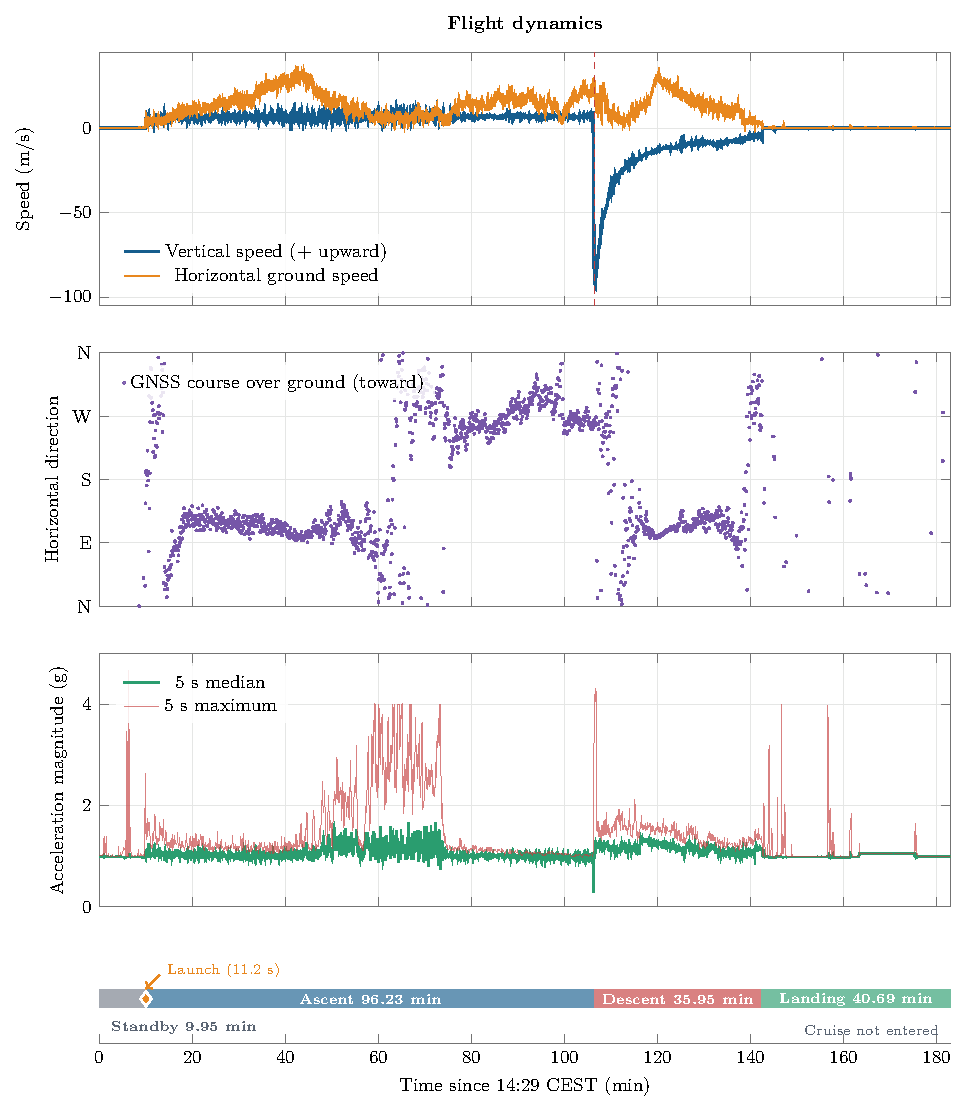
\includegraphics[width=\textwidth]{vertical_dynamics.pdf}
\caption{Flight dynamics.}
\label{fig:dynamics}
\end{figure}

Figure~\ref{fig:dynamics} compares GNSS vertical speed, horizontal ground speed,
and IMU acceleration magnitude. Positive vertical speed is upward. The red
acceleration trace retains the maximum value in each five-second plotting bin so
short peaks remain visible beside the median trend.

The maximum \MaxAccelerationG\ g magnitude occurred at \MaxAccelerationTime,
before the 14:38:56 Launch transition, with components $(1.548,-2.045,-3.909)$
g. It is therefore more likely associated with pre-launch handling or vehicle
dynamics than with balloon burst. The largest measured descent speed,
\MaxDescent\ m/s, occurred immediately after the apex transition and then
relaxed as the descent stabilised.

The 9.607 km altitude disagreement at apex is systematic rather than a single
sample spike: the two profiles diverge progressively during ascent and
reconverge during descent. Plausible contributors include the ground-relative
barometric reference, an inappropriate fixed atmosphere model, pressure-sensor
thermal behaviour, or model error in the very low pressure regime. Resolving
the cause requires recalculating altitude from raw pressure with the intended
reference pressure and comparing against GNSS altitude over pressure bands.

\section{Atmospheric measurements}

\begin{figure}[H]
\centering
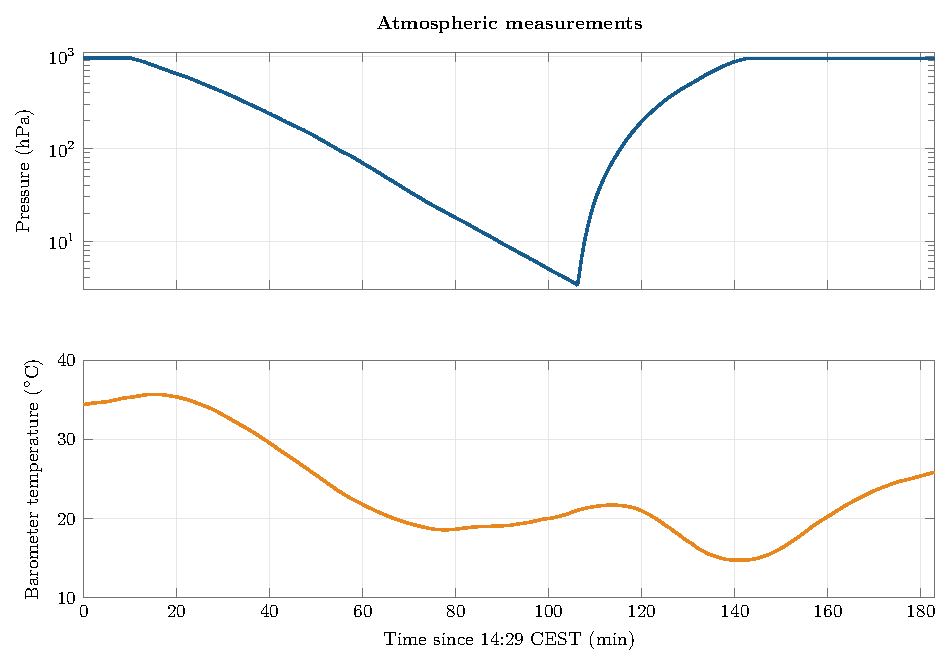
\includegraphics[width=\textwidth]{environment.pdf}
\caption{Atmospheric measurements.}
\label{fig:environment}
\end{figure}

Figure~\ref{fig:environment} uses ten-second medians and a logarithmic pressure
axis to show the large pressure range without obscuring the surface portions of
the flight. The MS5607 temperature trace is a sensor measurement used for
pressure compensation, not a direct ambient-air measurement.

Pressure decreased from roughly 957 hPa near the start of the window to a
minimum of \MinPressureHpa\ hPa near apex, then returned toward the surface
value. The logarithmic profile is smooth and physically consistent with the
gross altitude evolution; the main concern is the conversion from pressure to
reported relative altitude rather than continuity of the pressure measurement.

The reported barometer temperature ranged from \MinTemperatureC\ to
\MaxTemperatureC\ $^\circ$C. The channel changes smoothly, but its absolute
values should be interpreted as device temperature within the enclosure. It
cannot support an atmospheric lapse-rate conclusion without a separately
calibrated external temperature sensor and a thermal-lag model.

\section{GNSS trajectory}

\begin{figure}[H]
\centering
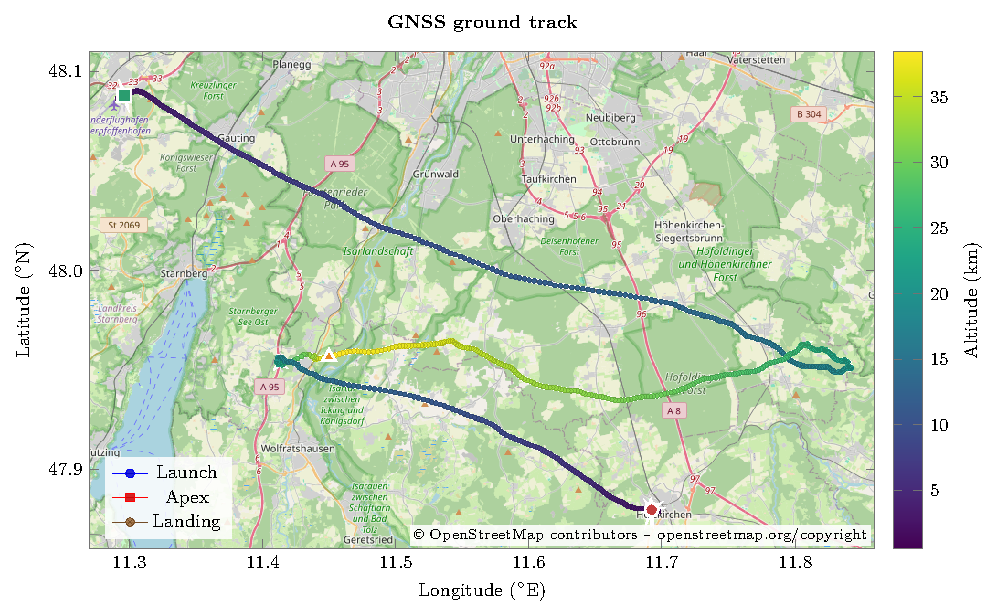
\includegraphics[width=0.92\textwidth]{trajectory.pdf}
\caption{GNSS ground track.}
\label{fig:trajectory}
\end{figure}

Figure~\ref{fig:trajectory} plots ten-second median GNSS positions over an
OpenStreetMap background in Web Mercator projection. Marker colour represents
GNSS altitude, while launch, apex, and landing are identified separately. Map
data: \copyright\ OpenStreetMap contributors,
\url{https://www.openstreetmap.org/copyright}.

\begin{table}[H]
\centering
\caption{GNSS event-position estimates.}
\label{tab:positions}
\begin{tabular}{@{}lrr@{}}
\toprule
Event & Latitude ($^\circ$N) & Longitude ($^\circ$E) \\
\midrule
Launch & \LaunchLatitude & \LaunchLongitude \\
Apex & \ApexLatitude & \ApexLongitude \\
Landing transition & \LandingLatitude & \LandingLongitude \\
\bottomrule
\end{tabular}
\end{table}

The great-circle launch-to-landing displacement is \LandingDistanceKm\ km; the
maximum range from the launch position during the window is \MaxRangeKm\ km.
These are point-to-point geodesic distances, not accumulated path length, so
they are not inflated by small GNSS position jitter.

The first 3D fix appears at \FirstFixTime\ CEST, \FirstFixMinutes\ minutes
after the start of the public window and before Launch. Prior coordinates in
the CSV are carried values without a usable 3D solution and are excluded from
the track and distance calculations.

\section{Electrical power and IMU observations}

\begin{figure}[H]
\centering
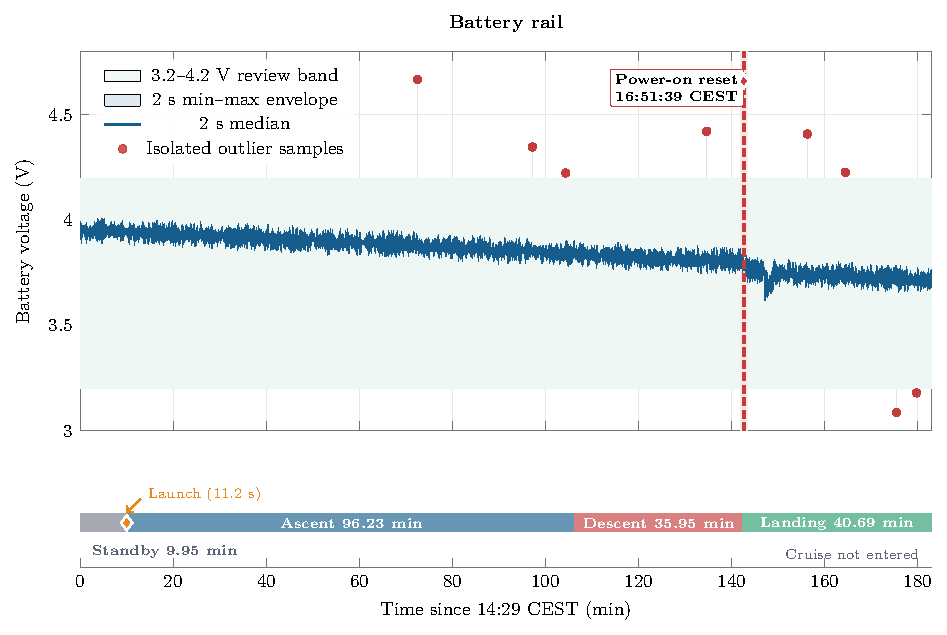
\includegraphics[width=\textwidth]{power_health.pdf}
\caption{Battery rail.}
\label{fig:power}
\end{figure}

Figure~\ref{fig:power} shows the battery trend, two-second extrema, and isolated
samples outside the 3.2--4.2~V review band. The power-on reset at 16:51:39 CEST
is marked by a red band, dashed line, diamond, and callout. The green band is an
analysis review threshold rather than a firmware-declared validity limit.

The battery median was \BatteryMedianV\ V, with a 5th--95th percentile range
of \BatteryPZeroFiveV--\BatteryPNinetyFiveV\ V. The full sample range was
\BatteryMinV--\BatteryMaxV\ V. Eight isolated rows fell outside the 3.2--4.2 V
review band. Each extreme is short relative to the sampling cadence and the
surrounding trend remains near the nominal rail, so the evidence favours ADC
or switching-transient glitches over sustained overvoltage or undervoltage.

The voltage trend gradually declined through flight and stepped downward after
the reboot, but the recorded battery-valid flag remained asserted throughout.
Because the reset cause is explicitly power-on rather than watchdog, the power
path, connector integrity, regulator undervoltage lockout, reset-cause capture,
and ADC/reference behaviour should be examined together.

\section{Coral payload results and link reliability}

\begin{figure}[H]
\centering
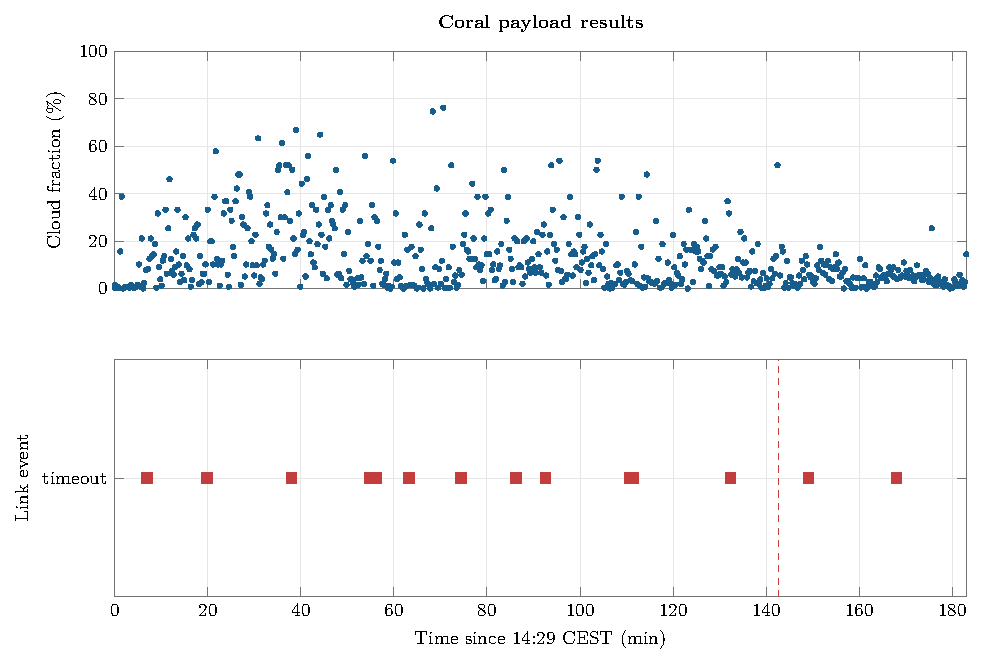
\includegraphics[width=\textwidth]{payload.pdf}
\caption{Coral payload results.}
\label{fig:payload}
\end{figure}

Figure~\ref{fig:payload} includes one point for each unique CRC-valid Coral
cloud-fraction result and one marker for each unique timeout record. Repeated
10~Hz copies of the same 16-byte receipt block are removed, and the dashed line
marks the OBC reboot.

The public window contains \GoodCoralFrames\ unique successful Coral results.
Their mean cloud fraction is \CloudMeanPercent\%, the median is
\CloudMedianPercent\%, and the 90th percentile is \CloudPNinetyPercent\%.
Approximately \CloudZeroPercent\% of successful results are exactly zero.
These are model outputs; without human-labelled imagery they describe the
payload response distribution, not independently verified cloud-cover truth.

The Coral channel was invalid for \CoralInvalidRows\ rows
(\CoralInvalidPercent\%) and carried timeout status for \CoralTimeoutRows\
rows. The equipment fault bit shows \CoralFaultIntervals\ distinct intervals,
totalling approximately \CoralTotalFaultS\ seconds of telemetry-tick duration;
the longest was \CoralLongestFaultS\ seconds during post-reset recovery. No
Coral CRC-error or Coral SD-error status was recorded.

Five in-window sequence omissions are adjacent to timeout intervals:
454$\rightarrow$456, 620$\rightarrow$622, 649$\rightarrow$651,
729$\rightarrow$731, and 816$\rightarrow$818. The firmware stores a RAW frame
only after a CRC-valid reception and deletes failed or partial frames.
Accordingly, the sequence gaps indicate discarded receptions, not proven
corruption of successfully stored image files.

\section{TT\&C downlink performance}

\begin{figure}[H]
\centering
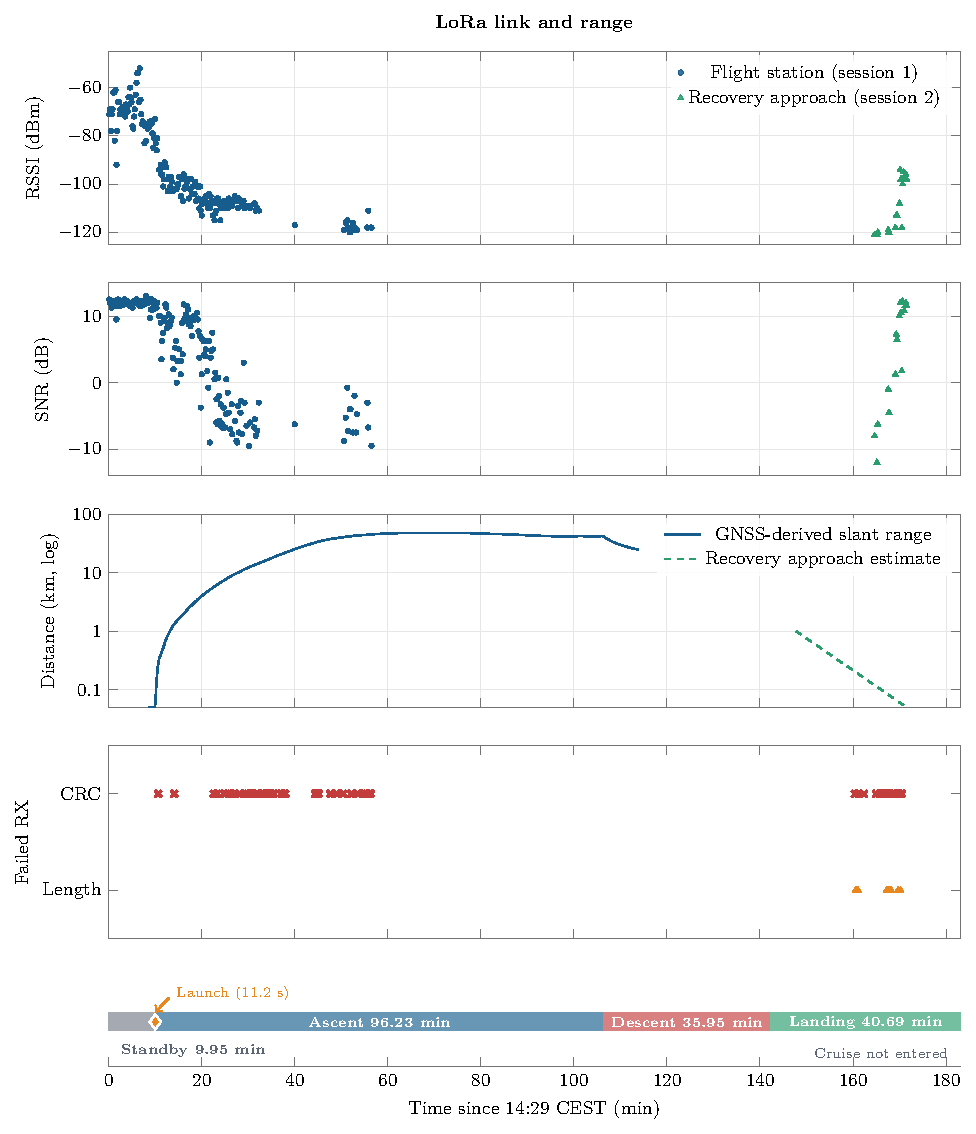
\includegraphics[width=\textwidth]{ttc_link.pdf}
\caption{LoRa link and range.}
\label{fig:ttc}
\end{figure}

Figure~\ref{fig:ttc} aligns RSSI, SNR, ground-station distance, and failed
receptions for the two LoRa sessions. The failure strip uses red crosses for
\TtcCrcErrorsInWindow\ CRC failures and orange triangles for
\TtcUnexpectedLengthPacketsInWindow\ unexpected-length receptions. Blank RSSI
or SNR spans contain no valid decoded packet and are not interpolated.

Within the public flight window, the ground logs contain \ValidDownlinks\ valid
decoded packets from \TtcFirstTime\ to \TtcLastTime\ CEST and
\TtcCrcErrorsInWindow\ LoRa CRC failures. The CRC failures represent
\InvalidDownlinkPercent\% of the \ValidDownlinks\ valid plus
\InvalidDownlinks\ CRC-failed telemetry reception rows. A further
\TtcUnexpectedLengthPacketsInWindow\ in-window receptions had unexpected
lengths and never entered the decoded telemetry table. Across the complete
ground-station sessions, including the period before the public flight window,
the corresponding counts are \TtcCrcErrors\ CRC failures and
\TtcUnexpectedLengthPackets\ unexpected-length packets. The valid packet
sequence fields report
\ReportedLostPackets\ packets lost since the previous reception and
\DuplicateDownlinks\ duplicates. Median RSSI was \RssiMedian\ dBm, spanning
\RssiMin\ to \RssiMax\ dBm; median SNR was \SnrMedian\ dB, spanning \SnrMin\
to \SnrMax\ dB.

For session 1, the ground station is modelled at the CubeSat's initial valid
GNSS position, consistent with the field setup, and held fixed. The resulting
3D slant range includes both horizontal separation and altitude difference.
The last valid reception occurred at approximately \SessionOneLastRangeKm\ km
slant range; by the later receiver stop the CubeSat was approximately
\SessionOneStopRangeKm\ km away. This supports range as an important contributor
to the observed progression from strong RSSI and positive SNR toward roughly
$-120$ dBm and negative SNR, although it does not isolate propagation,
orientation, or antenna effects.

The recovery station began session 2 at \SessionTwoStartTime\ CEST while the
CubeSat was stationary. No station GNSS track was logged, so the dashed distance
line is explicitly an estimate based on the operator account: the station began
about \SessionTwoStartRangeKm\ km away and approached the CubeSat, with
co-location assigned to the final valid packet at \SessionTwoEndTime\ CEST.
The renewed valid receptions and improving RSSI/SNR are consistent with the
shrinking range, but the distance curve must not be interpreted as a measured
trajectory. The logarithmic distance panel uses 0.05~km as a plotting floor at
co-location.

The main antenna was detached during this transmission configuration and the
radio radiated from the remaining feed cable. That non-standard radiator likely
had a poorly controlled impedance and radiation pattern and may have reduced or
made the effective radiated power strongly orientation-dependent. It is therefore
a plausible contributor to the CRC errors, unexpected packet lengths, and other
decode failures, together with range and propagation geometry; the logs cannot
quantify its causal share. The long blank region must also be interpreted
conservatively: these files describe what this ground station received, not every
radio transmission. The on-board \texttt{scv\_lora\_timeout\_count} and
\texttt{scv\_lora\_tx\_fault\_counter} remained zero, so the data do not show an
OBC-declared LoRa hardware fault.

\clearpage
\section{Recovery}

The state machine entered Landing at \LandingTime\ CEST. A power-on reset was
then observed at 16:51:39 CEST, but the first boot-6 record retained the Landing
state and the persisted mission time. This allowed post-landing operation to
continue without the software reverting to Standby. The cause of the
interruption remains unresolved and should not be treated as a nominal recovery
event.

The second ground-station session began at \SessionTwoStartTime\ CEST with the
station approximately \SessionTwoStartRangeKm~km from the stationary CubeSat.
The station approached the recovery point, and the range comparison assigns
co-location to the final valid packet at \SessionTwoEndTime\ CEST. Valid packets
reappeared and link quality improved as the estimated distance decreased,
supporting successful close-range reacquisition.

The main LoRa antenna was detached during this configuration, so the radio was
transmitting through the remaining feed cable. The cable was an uncontrolled
radiator, and its impedance, radiation pattern, and orientation were not known.
The recovery link therefore demonstrated that packets could still be received
at close range, but it was not a representative end-to-end validation of the
nominal antenna system. The lack of a logged station GNSS track also means that
the plotted recovery distance is an operational estimate rather than a
measurement.

\statusbox{lakituorange}{lightorange}{Recovery assessment. The CubeSat remained operational after landing and was reacquired during the station approach, but the power-on reset, detached antenna, and unlogged station trajectory limit the conclusions that can be drawn from the recovery link.}

\section{System health, FDIR, and reboot}

All records carry \texttt{scv\_equipment\_enabled}=127, meaning GPS, IMU,
barometer, Coral, SD, LoRa, and EPS ADC remained enabled. The only equipment
fault values are 0 and 8; bit 8 is the Coral fault. No row carries a GPS, IMU,
barometer, SD, LoRa, EPS, or CDH fault. The I2C recovery state is always zero.

The maxima of the recorded GPS, IMU, barometer, LoRa, LoRa-TX, SD, and watchdog
counters are all zero. GPS, IMU, barometer, and battery validity flags are each
asserted for 100\% of the primary rows. Coral is the sole channel with a
material validity interruption.

The last boot-5 row is followed by boot 6 after an observed GNSS-time gap of
\BootGapS\ seconds, with the first new record at 16:51:39 CEST.
\texttt{scv\_reset\_reason}=1 denotes a power-on reset. The watchdog reset
counter remains zero, and the persisted phase and mission elapsed time resume
in Landing. This demonstrates successful state persistence but leaves the
physical source of the power interruption unresolved.

\section{Data quality and limitations}

\begin{figure}[H]
\centering
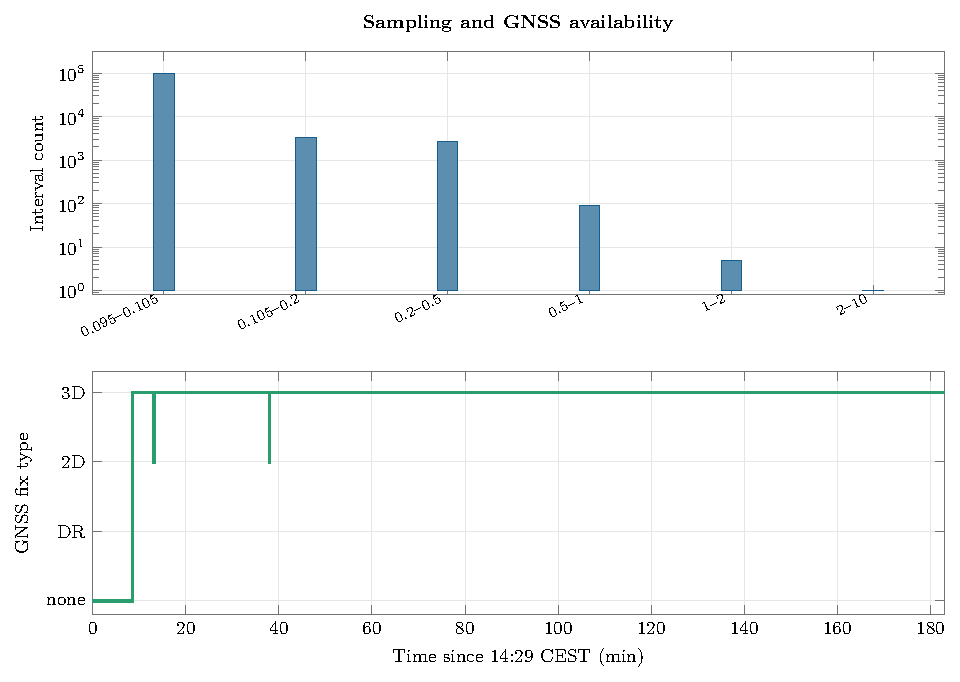
\includegraphics[width=\textwidth]{data_quality.pdf}
\caption{Sampling and GNSS availability.}
\label{fig:quality}
\end{figure}

Figure~\ref{fig:quality} combines the within-boot HAL-tick interval histogram
with GNSS fix type over the mission timeline. The histogram excludes the boot
boundary so the reset gap is not misclassified as a sampling stall.

The median within-boot sample interval is \MedianSampleMs\ ms and the 95th
percentile is \SamplePNinetyFiveMs\ ms. Six intervals are at least one second:
five genuine stalls between 1.0 and \LongestGenuineStallS\ seconds plus one
8.673-second artefact caused by the public-cut filter. The full archive contains
81 valid rows in that interval, but their \texttt{gps\_utc\_time} is zero and
they were excluded when the public file was selected by non-zero GNSS clock.
No archive CSV-file sequence gap or within-boot gap above two seconds is
reported by the full audit.

GNSS transport validity is 100\%, while a 3D navigation fix is present for
\FixThreeRows\ rows (\FixThreePercent\%). The distinction is important:
\texttt{gps\_valid}=1 means the receiver data are fresh and accepted; it does
not mean a usable 3D solution. The initial no-fix interval ends at
\FirstFixTime, and three later 2D/no-fix interruptions are brief.

The following limitations govern interpretation:

\begin{itemize}
  \item The GNSS calendar date is an archive assumption; only time of day is stored on board.
  \item The public CSV omits the 81 GNSS-time-zero rows; continuity conclusions use the full archive audit.
  \item Barometric altitude is relative and model-dependent. Raw pressure is the more direct observable.
  \item Barometer temperature is an internal sensor measurement, not validated ambient temperature.
  \item Cloud fractions have no manual ground-truth labels in the released dataset.
  \item Ground-station link logs are receive-side samples; missing receptions do not identify a unique failure cause.
  \item Session 2 ground-station distance is an operator-informed linear estimate because no station GNSS track was recorded.
  \item Five- or ten-second medians are used only for graph readability. Summary extrema use full-rate rows.
\end{itemize}

\section{Lessons learnt}

\begin{enumerate}
  \item \textbf{Persistent, multi-sensor logging made the flight reconstructable.}
  The 10~Hz on-board record, boot counter, state, reset reason, and validity
  fields allowed the flight timeline to be recovered even across the reboot.
  \item \textbf{State persistence is valuable, but power continuity is still a
  single-point concern.} Restoring Landing after the reset prevented an unsafe
  state regression; it did not remove the need to identify the physical power
  interruption.
  \item \textbf{A validity flag is not the same as measurement plausibility.}
  The barometric channel remained valid despite its large high-altitude
  disagreement with GNSS, and isolated battery ADC outliers passed the recorded
  validity logic.
  \item \textbf{Receive-side TT\&C data need configuration and geometry context.}
  Range, station motion, antenna attachment, cable configuration, and orientation
  must be logged alongside RSSI and SNR before decode failures can be attributed
  to a specific cause.
  \item \textbf{Payload fault flags identified the affected subsystem but not
  the mechanism.} Coral timeouts were visible and recovered automatically, yet
  the available fields cannot distinguish framing, buffering, UART, or payload
  response delays.
  \item \textbf{Flight-state names must be checked against mission intent.} The
  direct Ascent-to-Descent transition was consistent with the implemented rule
  order, but Cruise was never entered. Requirements and transition priority
  should agree before the next flight.
\end{enumerate}

\clearpage
\section{Future work}

Recommended actions before the next flight, in priority order, are:

\begin{enumerate}
  \item \textbf{Investigate the power-on reset.} Inspect battery and regulator logs, connector retention, UVLO thresholds, brownout configuration, reset-cause capture, and the timing relationship between voltage transients and reboot.
  \item \textbf{Harden the Coral UART path.} Correlate each timeout with receive-state diagnostics, buffer high-water marks, SD activity, and frame duration. Add explicit per-attempt outcome logging so missing sequences can be attributed without inference.
  \item \textbf{Recalibrate barometric altitude.} Recompute altitude from pressure using a documented reference pressure and atmosphere model; compare residuals against GNSS altitude versus pressure, temperature, and ascent/descent direction.
  \item \textbf{Validate EPS ADC sampling.} Reproduce switching loads on the bench, inspect reference and divider settling, and add filtering or plausibility rejection for isolated samples outside the electrical design envelope.
  \item \textbf{Repeat the TT\&C link test.} Reattach and tune the main antenna, measure return loss, log ground-station GNSS, and repeat controlled range and orientation steps so antenna and propagation effects can be separated.
  \item \textbf{Review FSM requirements.} Confirm whether skipping Cruise is acceptable. If Cruise is required, test transition ordering and persistence conditions against the observed apex profile.
  \item \textbf{Unify the public analysis master.} Restore or explicitly join the 81 GNSS-time-zero rows using boot count and HAL tick so downstream users do not mistake a selection artefact for a logging outage.
\end{enumerate}

\section{Conclusions}

The public flight record is coherent and supports a defensible reconstruction
of pre-flight Standby, launch, ascent, burst/descent, landing, and recovery
operations. Core GPS, IMU, barometer, battery, I2C, SD, and LoRa health remained
nominal from the flight software's perspective. The most consequential findings
are the Coral timeout recurrence, the mid-landing power-on reset, the
high-altitude barometric/GNSS disagreement, and the limited interpretability of
the recovery link with the main antenna detached. The platform's persistent
state and detailed logging worked well; closing the identified power, payload,
measurement-validation, and test-traceability gaps should be the priority for
the next campaign.

\appendix
\section{Reproducibility}

Run the following from the repository root on a system with Node.js and TeX
Live (including \texttt{latexmk}, PGFPlots, and Poppler):

\begin{verbatim}
powershell -ExecutionPolicy Bypass -File flight-data/report/build_report.ps1
\end{verbatim}

The build performs four stages: regenerates the numerical summary and compact
CSVs, compiles each standalone vector graph, compiles this report, and copies
the final PDF to \sourcefile{output/pdf/Lakitu_Flight_Data_Report.pdf}.

The machine-readable summary is
\sourcefile{flight-data/report/analysis_summary.json}. The plot-driving CSVs
are in \sourcefile{flight-data/report/processed/}. They are derived artefacts;
the original flight-data files remain unchanged.

\section{Input checksums}

\scriptsize
\begin{longtable}{@{}p{0.31\textwidth}p{0.64\textwidth}@{}}
\toprule
Input & SHA-256 \\
\midrule
\endhead
Public flight window & \ttfamily 0cbe579b5d2ecc1186afbdbc2a8ac285f2cfefe9db8a2e221402e52489cc7ea0 \\
Full archive CSV & \ttfamily ebad4569d5744696ed02636cfecc19c88a1d810e2ea28003309a15cdf56aeb3d \\
Ground telemetry session 1 & \ttfamily e734fff42dad4bd7825452d655f964e40afc276da179c462f246623c29bff3cd \\
Ground telemetry session 2 & \ttfamily c85d80ade6346218438a46a059148746bfbfb9ff5eed71634be2f6826bbf8e31 \\
\bottomrule
\end{longtable}
\normalsize

\end{document}
